\section{Recovering the sofa; proof of Theorem~\ref{thm:main}}\label{sec:recovery}

By \eqref{eq:contained} and \cref{thm:caps}, a rigid image of $S$ lies in a horizontal translate of $\Gs$ and has
the same area. A closed subset of a set of finite area, with the same area, is the whole set if that set
is the closure of its interior (\cref{lem:recover}), but not in general (\cref{fig:recovery}, Remark~\ref{rem:needed}). So it remains to show that $\Gs$ is.

\begin{lemma}[recovering a set from its area]\label{lem:recover}
Let $X\subset Y\subset\R^2$ with $X$ closed, $Y=\clos(\inter Y)$, $\abs Y<\infty$ and $\abs X=\abs Y$. Then $X=Y$.
\end{lemma}

\begin{proof}
$\abs{Y\setminus X}=0$. The set $\inter Y\setminus X$ is open, and it has measure $0$, so it is empty. Hence
$\inter Y\subset X$, and since $X$ is closed, $Y=\clos(\inter Y)\subset X$.
\end{proof}

\begin{remark}\label{rem:needed}
Both hypotheses on $Y$ are needed. The closed connected set $Y=[0,1]^2\cup([1,2]\times\{0\})$ and its closed
subset $X=[0,1]^2$ have the same finite area, and $Y$ is not the closure of its interior. For $Y=\R^2$ and $X=\R^2$ minus the open unit disc, $Y=\clos(\inter Y)$ and
$\abs X=\abs Y=\infty$. For $Y=\Gs$, a closed subset that misses an interior point of $\Gs$ misses a disc about it, and so loses area.
\end{remark}

\begin{lemma}[removing the region under an envelope]\label{lem:envelope}
Let $K\subset\R^2$ be closed with $K=\clos(\inter K)$ and $[a,b]\times[0,1]\subset K$. Let $\Gamma$ be a compact set of points with
abscissa in $[a,b]$ and height in $[0,1)$, and let $\Gamma_<$ be the set of points $q$ with $q_y\ge0$ that lie strictly
below a point $\gamma$ of $\Gamma$ with $\gamma_x=q_x$. If $X=K\setminus\Gamma_<$ is closed, then $X=\clos(\inter X)$.
\end{lemma}

\begin{proof}
Let $\bar\Gamma$ be the set of points $q$ with $q_y\ge0$ that lie on or below a point of $\Gamma$ with the same abscissa; it
is the image of the compact set $\Gamma\times[0,1]$ under $(\gamma,\lambda)\mapsto(\gamma_x,\lambda\gamma_y)$, hence compact, and
$\Gamma_<\subset\bar\Gamma$. Let $p\in X$.

If $p\notin\bar\Gamma$, then $p$ has a neighborhood outside $\bar\Gamma$, and since $K=\clos(\inter K)$ it is a limit of interior
points of $K$ outside $\bar\Gamma$; these are interior points of $X=K\setminus\Gamma_<$. So $p\in\clos(\inter X)$.

If $p\in\bar\Gamma$, then $p\notin\Gamma_<$ means that $p$ is the highest point of $\Gamma$ on its vertical line: $p_x\in[a,b]$ and
$p_y<1$. The points $(p_x,p_y+s)$, $0<s\le1-p_y$, lie in the rectangle $[a,b]\times[0,1]\subset K$ and outside $\bar\Gamma$, so by the
first case they lie in $\clos(\inter X)$, and so does their limit $p$.

So $X\subset\clos(\inter X)$, and $\clos(\inter X)\subset X$ since $X$ is closed.
\end{proof}

\begin{proposition}[Gerver's sofa is regular closed]\label{prop:regular}
$\Gs=\clos(\inter\Gs)$.
\end{proposition}

\begin{proof}
Let $\Gamma=\bD([t_0,t_2])\cup\xx([t_1,t_4])\cup\bB([t_3,t_5])$, $a=\bD(0)_x$ and $b=\bB(\pi/2)_x$. By
\cref{fact:gerver}\ref{fact:gerver:cap} and~\ref{fact:gerver:niche}, $\Gs=\KG\setminus\cN(\KG)=\KG\setminus\Gamma_<$, which is closed, being a moving sofa.
The set $\Gamma$ is compact. The abscissa increases along $\bD$ and $\bB$ and, as $t$ grows, decreases along $\xx$, and the
endpoints are joined, so
\[
  a=\bD(0)_x<\bD(t_2)_x=\xx(t_4)_x<\xx(t_1)_x=\bB(t_3)_x<\bB(t_5)_x=b ,
\]
and the abscissa of every point of $\Gamma$ lies in $[a,b]$. The ordinate of $\bD$ is nondecreasing, since
$\bD'$ is a positive multiple of $u_t$ and $\sin t\ge0$; it starts at $0$ and ends at $\xx(t_4)_y<1$. The ordinate of $\bB$ is
nonincreasing, since $\bB'$ is a negative multiple of $v_t$; it ends at $0$ and starts at $\xx(t_1)_y<1$. The ordinate of $\xx$ on
$[t_1,t_4]$ lies in $(0,1)$ by \cref{fact:height}. So the heights of $\Gamma$ lie in $[0,1)$.

The points $(a,1)=\bD(0)+v_0=\bC(0)$ and $(b,1)=\bB(\pi/2)+u_{\pi/2}=\bA(\pi/2)$ are vertices of the cap $\KG$ (\cref{fact:gerver}\ref{fact:gerver:cap}), so they lie in $\KG$.
A cap with rotation angle $\pi/2$ is closed downward above the floor: for $p\in K$ and $0\le\lambda\le p_y$ we have $p-(0,\lambda)\in K$,
because $\ip{(0,-\lambda)}{u_s}\le0$ for $s\in[0,\pi]$. Hence $\KG\supset[a,b]\times[0,1]$, so $\KG$ is a closed convex set with nonempty interior, and
$\KG=\clos(\inter\KG)$. \cref{lem:envelope} applies with $K=\KG$.
\end{proof}

\begin{figure}[ht]
\centering
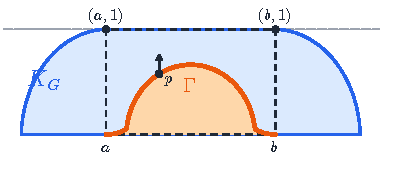
\includegraphics[width=0.92\linewidth]{figures/fig-recovery}
\caption{\cref{prop:regular}. Left: Gerver's cap $\KG$ with its niche (orange) below the curve $\Gamma$ formed by $\bD$, $\xx$ and $\bB$; the dashed rectangle
$[a,b]\times[0,1]$ lies in $\KG$, and the greatest height of $\Gamma$ is $0.664\ldots$. Every point $p$ of $\Gamma$ is a limit of points of
$\Gs$ above it. Right: why $\clos(\inter Y)=Y$ is needed in \cref{lem:recover}: a closed subset of $Y$ with the same area misses
no interior point.}
\label{fig:recovery}
\end{figure}

\begin{proof}[Proof of \cref{thm:main}]
Let $S$ be a moving sofa with $\abs S=\abs\Gs$. By \cref{prop:reduction}, \cref{prop:U} and \cref{thm:caps}, there are $\omega\in[\omega_0,\pi/2]$,
$\psi=\pi/2-\omega$, $w_0,w_1\in\R^2$ and $s\in\R$ such that
\[
  g_1(S)\subset U=\Gs+(s,0),\qquad g_1(p)=R_\psi(p+w_0)+w_1 .
\]
Let $g(p)=g_1(p)-(s,0)=R_\psi p+v$ with $v=R_\psi w_0+w_1-(s,0)$. Then $g(S)\subset\Gs$. The set $g(S)$ is closed, since $S$ is closed and $g$ is a
homeomorphism, and $\abs{g(S)}=\abs S=\abs\Gs<\infty$ since $g$ preserves area. By \cref{prop:regular}, $\Gs=\clos(\inter\Gs)$, so
$g(S)=\Gs$ by \cref{lem:recover}, that is, $R_\psi S+v=\Gs$. This is the assertion with $\theta=\psi$.
\end{proof}

The proof also gives the following description of all maximal sofas.

\begin{corollary}[the maximal sofas]\label{cor:all}
A set $S$ is a moving sofa of maximal area if and only if it is a moving sofa and $R_\theta S+v=\Gs$ for some $\theta$ and $v$.
\end{corollary}

\begin{proof}
One direction is \cref{thm:main} together with $\abs S=\abs\Gs$ being the maximum (\cref{fact:optimal}). Conversely a rigid image of $\Gs$ has the area of $\Gs$.
\end{proof}

\begin{remark}[no rotation is needed]\label{rem:translate}
In \cref{thm:main} one can take $\theta=0$: every moving sofa $S$ with $\abs S=\abs\Gs$ is a translate of $\Gs$, and so has the rotation angle $\pi/2$. This refinement is
not part of the formal statement. Indeed, a moving sofa lies after a translation in the strip $\R\times[0,1]$, so
$\abs{\ip{p-q}{u_{\pi/2}}}\le1$ for $p,q\in S$. In the proof above $\theta=\psi\in[0,\pi/2-\omega_0]$ and $S=R_{-\psi}(\Gs-v)$, so the width of $\Gs$ in the direction $u_{\pi/2+\psi}$ is at most one.
But the width of $\Gs$ in the direction $u_r$ exceeds one for every $r\in[0,\pi]\setminus\{\pi/2\}$, and $\pi/2+\psi\in[\pi/2,\pi)$; so $\psi=0$.

To see the claim about the width, let $a<b$ be as in \cref{prop:regular}, and let $x_-=\bC(\pi/2)_x$. The points $(a,1)=\bC(0)$ and $(b,1)=\bA(\pi/2)$ (the ends of the top edge of $\KG$), $(1,0)=\bA(0)$ (Appendix~\ref{app:gerver}, condition~(2))
and $(x_-,0)=\bC(\pi/2)$ (the ends of the floor, by \eqref{eq:ends}, \cref{fact:arms}\ref{fact:arms:regular} and \cref{fact:gerver}\ref{fact:gerver:cap}) lie in $\KG$, and not in $\cN(\KG)$: the points of $\cN(\KG)$ have height less than $1$ and abscissa in $(a,b)$ (the
only points of $\Gamma$ with abscissa $a$ or $b$ are $\bD(t_0)$ and $\bB(t_5)$, of height $0$), while $x_-=-h_{\KG}(\pi)\le a<b\le h_{\KG}(0)=1$. So they lie in $\Gs$.
For $r\in[0,\pi/2)$ the width of $\Gs$ in the direction $u_r$ is at least $\ip{(b,1)-(x_-,0)}{u_r}=(b-x_-)\cos r+\sin r>\cos r+\sin r\ge1$, because $b-x_->1$: indeed $x_-=\bC(\pi/2)_x=\xx(\pi/2)_x-1$, and
$b=\bB(t_5)_x>\bB(t_3)_x=\xx(t_1)_x>\xx(t_4)_x\ge\xx(\pi/2)_x$ by \cref{fact:gerver}\ref{fact:gerver:niche}.
For $r\in(\pi/2,\pi]$ it is at least $\ip{(a,1)-(1,0)}{u_r}=(1-a)\abs{\cos r}+\sin r>\abs{\cos r}+\sin r\ge1$, because $a<0$:
$a=\bD(t_0)_x<\bD(t_2)_x=\xx(t_4)_x<\xx(t_1)_x\le\xx(0)_x=0$ by \cref{fact:gerver}\ref{fact:gerver:niche} and Appendix~\ref{app:gerver}, condition~(2).
(Numerically, $a=-1.4206\ldots$, $b=0.1931\ldots$ and $x_-=-2.2275\ldots$.)
\end{remark}
